\begin{figure*}[ht]
  \centering
  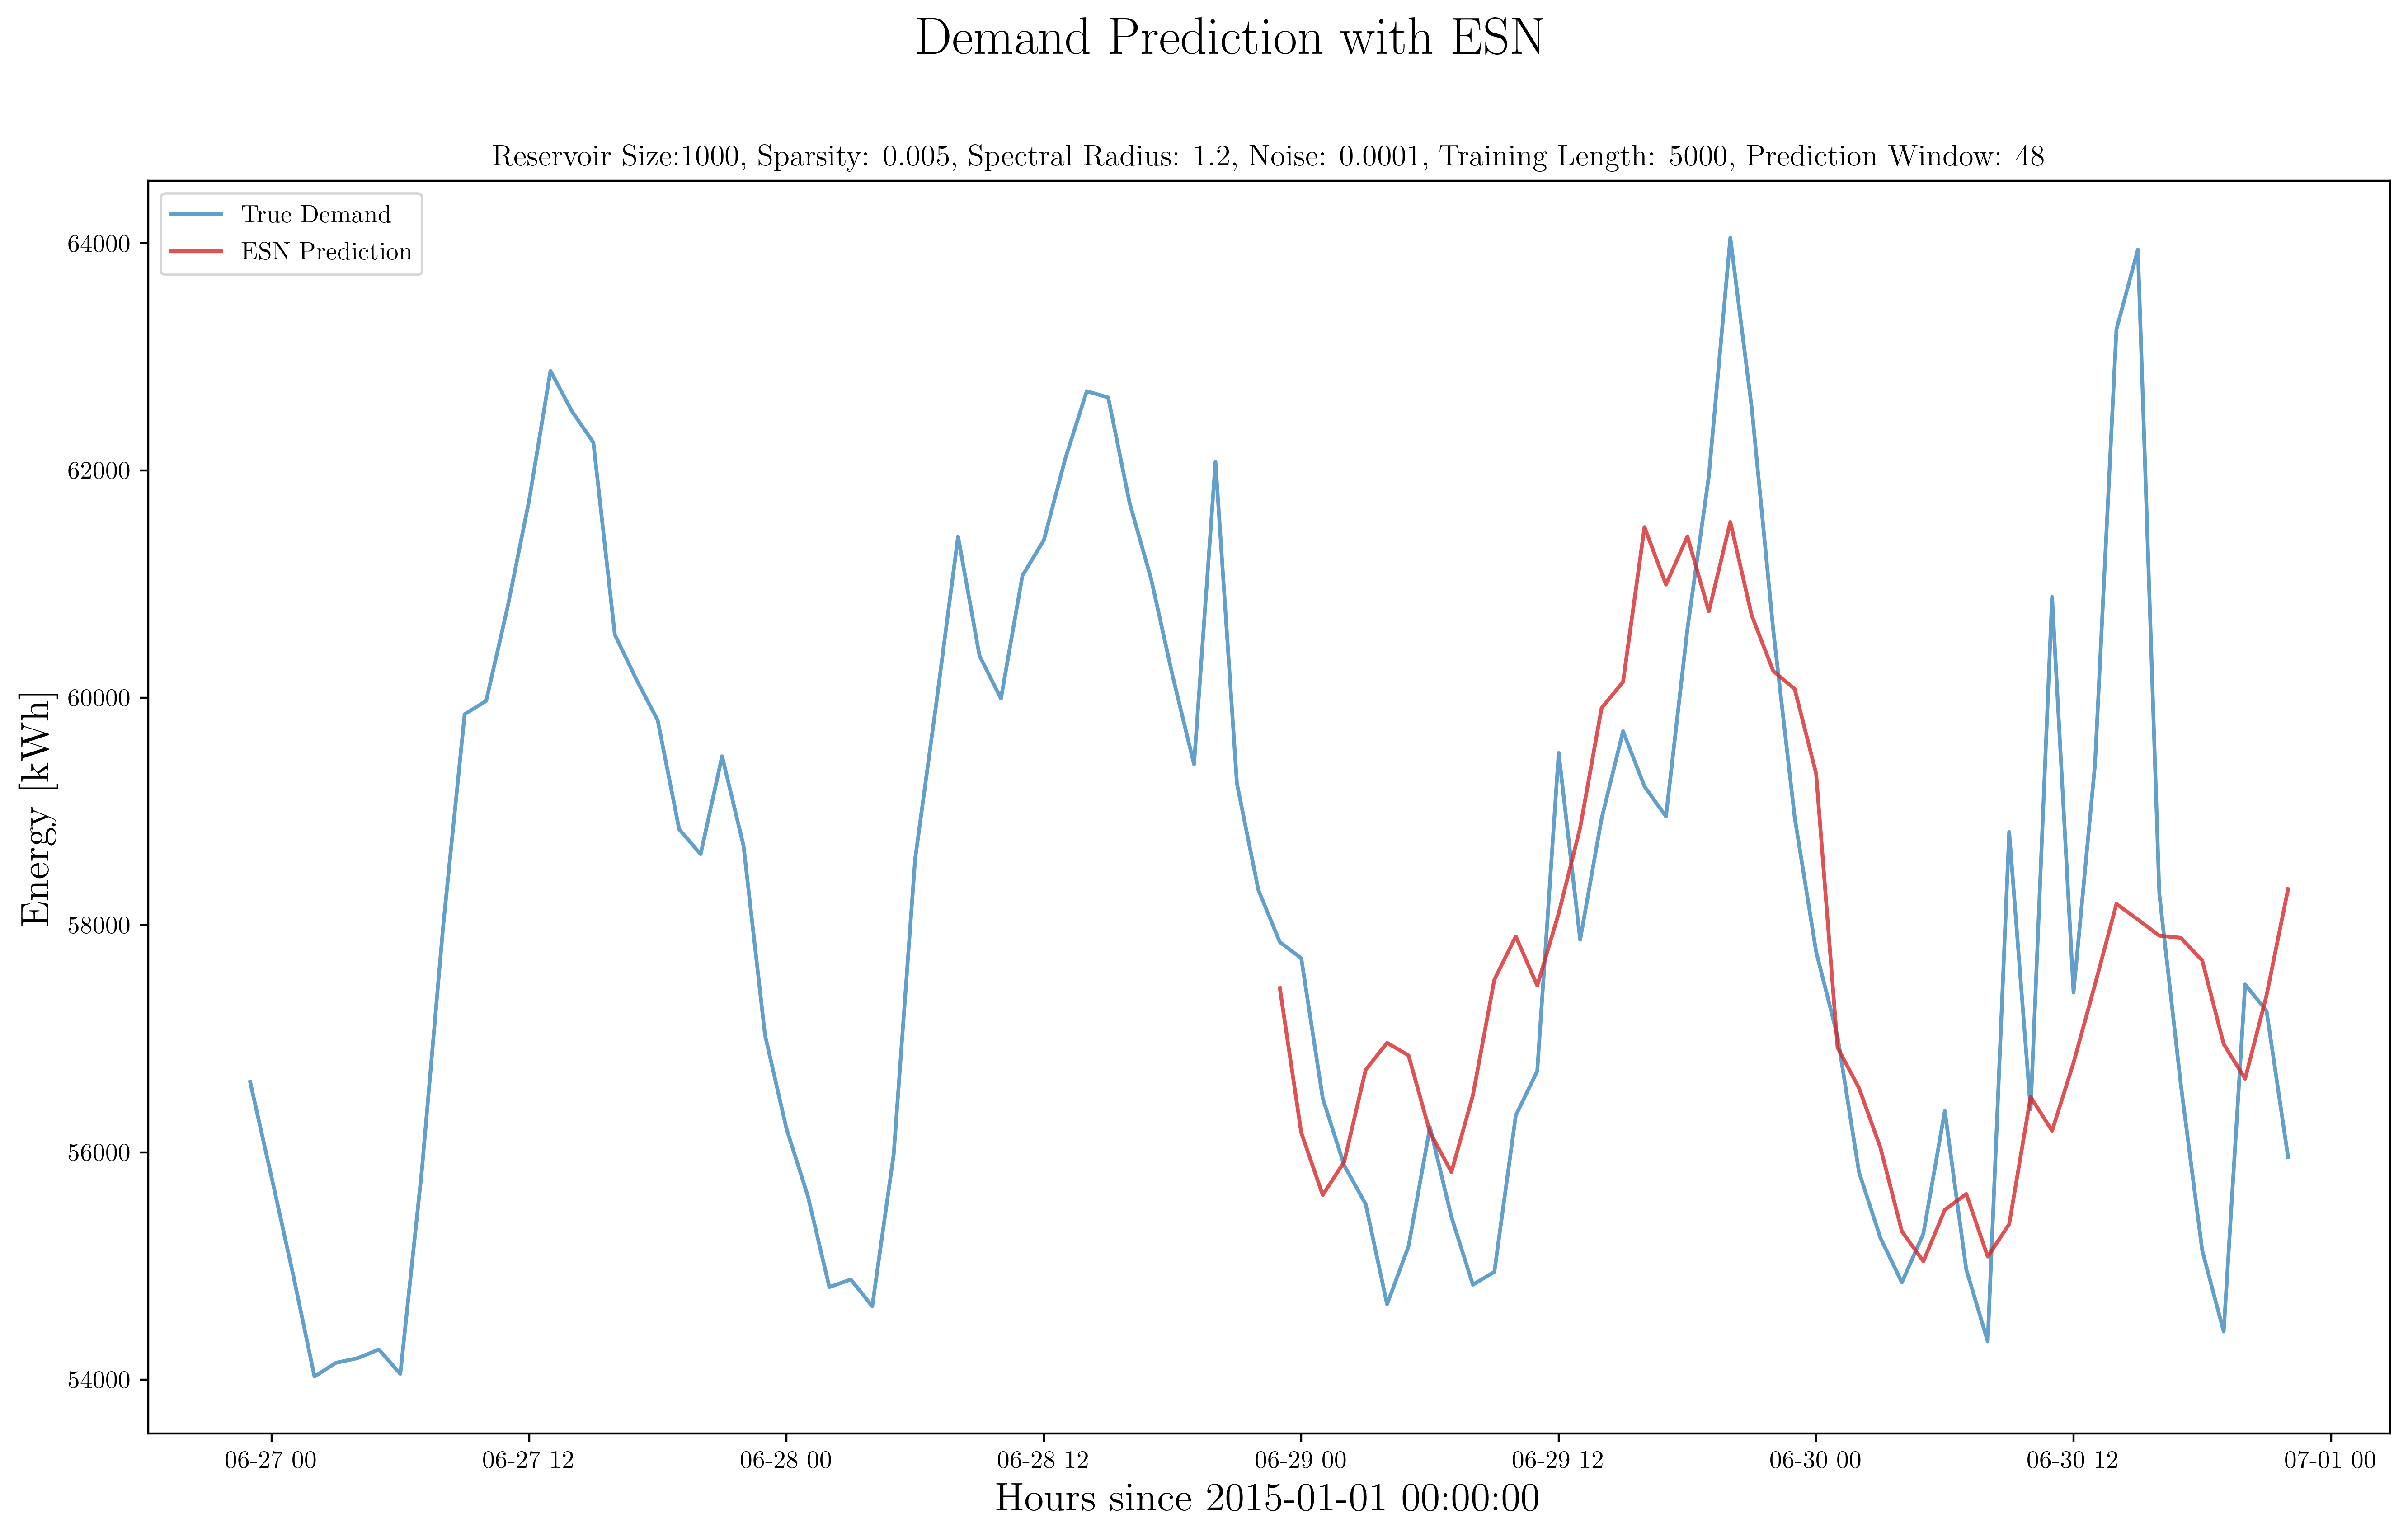
\includegraphics[width=0.8\textwidth]{48_demand_pressure_prediction.png}
  \caption{The optimized 48-hour ahead demand prediction with pressure as a  meteorological
  predictor.}
  \label{fig:48demand}
\end{figure*}

% \begin{center}
  \begin{table*}[ht]
    \centering
    \caption{Tabulated error for 48-hour ahead total electricity demand forecasts with various coupled quantities. Improvement indicates the percentage improvement over the base case of forecasting electricity demand alone.}
    \label{tab:demand48}
    \begin{tabular}{l|c|c|c|c}
      &  & & Improvement & Improvement \\
      Scenario  & MAE & RMSE & MAE (\%) & RMSE (\%)\\
      \hline
      Total Demand & 0.018892 & 0.024137 & [-] & [-] \\
      Demand + Sun Elevation & 0.013375 & 0.022893 & -29.20& -5.15 \\
      Demand + Humidity & 0.048357 & 0.063544 & +155.96 & +163.26 \\
      Demand + Pressure & 0.009329 & 0.017334 & -50.62 & -28.18\\
      Demand + Wet Bulb Temp. & 0.033473 & 0.039922 & +77.18 & +65.40\\
      Demand + Dry Bulb Temp. & 0.031866 & 0.040409 & +66.67 & +67.42\\
      Demand + Wind Speed & 0.051045 & 0.074966 & +170.19 & +210.58\\
    \end{tabular}
  \end{table*}
% \end{center}
